% !TEX program = lualatex
% !TEX encoding = UTF-8 Unicode
% !TEX spellcheck = de_DE
% 
% © 2015–2017 Moritz Brinkmann, CC-by-sa
% http://latexkurs.github.io

\documentclass[
	vorläufig=false,
	datum=2018-11-26,
	titel={Diagramme},
	web=false,
%	noshortverb=true,
	max,
	aspectratio=1610,
]{../tex/latexkurs-slides}

\usepackage{
	booktabs,
	filecontents,
	pgfplots,
}

\pgfplotsset{
	compat=1.16,
	width=7cm,
	lua backend=true,
}

\begin{filecontents}{data.dat}
time	values	error
0.00E+00	6.66E+01	7.85E-01
1.00E-01	4.69E+01	8.39E-01
2.00E-01	4.61E+01	1.33E+00
3.00E-01	5.87E+01	7.20E-01
4.00E-01	3.95E+01	1.75E+00
5.00E-01	5.47E+01	7.41E-01
6.00E-01	5.82E+01	6.22E-01
7.00E-01	4.26E+01	2.01E+00
8.00E-01	4.74E+01	8.85E-01
9.00E-01	5.75E+01	1.38E+00
1.00E+00	4.23E+01	1.75E+00
1.10E+00	4.10E+01	4.96E-01
1.20E+00	5.20E+01	9.71E-01
1.30E+00	4.14E+01	6.39E-01
1.40E+00	5.74E+01	1.71E+00
1.50E+00	6.74E+01	1.73E+00
1.60E+00	3.67E+01	1.88E+00
1.70E+00	4.57E+01	2.04E+00
1.80E+00	5.53E+01	1.76E+00
1.90E+00	5.36E+01	1.01E+00
2.00E+00	3.67E+01	1.71E+00
2.10E+00	4.77E+01	1.44E+00
2.20E+00	2.07E+01	1.21E+00
2.30E+00	4.21E+01	1.61E+00
2.40E+00	4.90E+01	1.24E+00
2.50E+00	2.95E+01	4.23E-01
2.60E+00	4.34E+01	7.34E-01
2.70E+00	5.01E+01	1.42E+00
2.80E+00	5.67E+01	2.00E+00
2.90E+00	4.16E+01	1.25E+00
3.00E+00	6.37E+01	1.14E+00
3.10E+00	5.19E+01	7.79E-01
3.20E+00	6.52E+01	1.09E+00
3.30E+00	4.72E+01	8.79E-01
3.40E+00	5.12E+01	2.29E+00
3.50E+00	4.09E+01	1.70E+00
3.60E+00	4.37E+01	1.14E+00
3.70E+00	5.63E+01	6.61E-01
3.80E+00	4.46E+01	1.79E+00
3.90E+00	4.47E+01	1.21E+00
4.00E+00	4.84E+01	1.55E+00
4.10E+00	5.31E+01	1.25E+00
4.20E+00	4.73E+01	1.56E+00
4.30E+00	4.47E+01	8.65E-01
4.40E+00	5.69E+01	1.49E+00
4.50E+00	5.10E+01	1.16E+00
4.60E+00	4.61E+01	9.93E-01
4.70E+00	5.39E+01	1.27E+00
4.80E+00	5.66E+01	6.96E-01
4.90E+00	5.48E+01	1.28E+00
5.00E+00	6.04E+01	1.01E+00
5.10E+00	5.96E+01	6.92E-01
5.20E+00	4.86E+01	2.09E+00
5.30E+00	6.14E+01	3.53E+00
5.40E+00	4.09E+01	6.52E-01
5.50E+00	3.89E+01	9.98E-01
5.60E+00	5.00E+01	1.06E+00
5.70E+00	3.54E+01	4.91E-01
5.80E+00	5.30E+01	1.25E+00
5.90E+00	3.34E+01	1.57E+00
6.00E+00	4.61E+01	1.20E+00
6.10E+00	4.18E+01	1.96E+00
6.20E+00	5.91E+01	6.14E-01
6.30E+00	3.65E+01	4.75E-01
6.40E+00	4.36E+01	5.77E-01
6.50E+00	5.05E+01	2.57E+00
6.60E+00	5.72E+01	1.23E+00
6.70E+00	3.58E+01	2.03E+00
6.80E+00	4.99E+01	5.78E-01
6.90E+00	2.99E+01	1.31E+00
7.00E+00	5.19E+01	7.83E-01
7.10E+00	6.05E+01	1.35E+00
7.20E+00	5.34E+01	1.65E+00
7.30E+00	6.39E+01	1.14E+00
7.40E+00	3.87E+01	8.47E-01
7.50E+00	5.40E+01	1.37E+00
7.60E+00	2.81E+01	1.95E+00
7.70E+00	4.92E+01	1.38E+00
7.80E+00	5.91E+01	1.81E+00
7.90E+00	4.31E+01	7.86E-01
8.00E+00	5.29E+01	1.26E+00
8.10E+00	5.58E+01	1.22E+00
8.20E+00	4.53E+01	9.30E-01
8.30E+00	4.91E+01	1.17E+00
8.40E+00	3.61E+01	1.20E+00
8.50E+00	5.85E+01	1.28E+00
8.60E+00	5.56E+01	9.99E-01
8.70E+00	4.01E+01	1.52E+00
8.80E+00	5.43E+01	5.87E-01
8.90E+00	4.71E+01	2.04E+00
9.00E+00	6.66E+01	9.54E-01
9.10E+00	6.56E+01	8.88E-01
9.20E+00	4.63E+01	1.31E+00
9.30E+00	4.37E+01	6.35E-01
9.40E+00	3.41E+01	1.48E+00
9.50E+00	4.31E+01	1.69E+00
9.60E+00	5.13E+01	9.08E-01
9.70E+00	5.78E+01	6.10E-01
9.80E+00	4.35E+01	5.23E-01
9.90E+00	4.56E+01	2.18E+00
1.00E+01	3.93E+01	1.87E+00
1.01E+01	3.78E+01	1.04E+00
1.02E+01	5.35E+01	7.32E-01
1.03E+01	3.84E+01	5.04E-01
1.04E+01	3.86E+01	3.05E+00
1.05E+01	5.82E+01	6.16E-01
1.06E+01	5.76E+01	8.33E-01
1.07E+01	4.81E+01	4.92E-01
1.08E+01	4.80E+01	1.58E+00
1.09E+01	5.20E+01	1.09E+00
1.10E+01	5.62E+01	1.78E+00
1.11E+01	5.22E+01	7.71E-01
1.12E+01	6.96E+01	9.44E-01
1.13E+01	4.42E+01	3.20E+00
1.14E+01	5.85E+01	1.24E+00
1.15E+01	5.72E+01	8.41E-01
1.16E+01	4.46E+01	5.64E-01
1.17E+01	4.10E+01	4.68E-01
1.18E+01	4.83E+01	2.23E+00
1.19E+01	4.77E+01	1.56E+00
1.20E+01	4.03E+01	1.33E+00
1.21E+01	4.50E+01	2.55E+00
1.22E+01	5.07E+01	1.56E+00
1.23E+01	5.84E+01	8.86E-01
1.24E+01	6.17E+01	6.23E-01
1.25E+01	5.66E+01	2.86E+00
1.26E+01	4.94E+01	7.67E-01
1.27E+01	4.58E+01	1.72E+00
1.28E+01	3.01E+01	1.95E+00
1.29E+01	5.98E+01	9.92E-01
1.30E+01	3.92E+01	5.37E-01
1.31E+01	5.37E+01	1.58E+00
1.32E+01	6.17E+01	1.34E+00
1.33E+01	5.46E+01	1.57E+00
1.34E+01	5.49E+01	1.28E+00
1.35E+01	4.73E+01	6.21E-01
1.36E+01	4.93E+01	1.26E+00
1.37E+01	6.05E+01	2.27E+00
1.38E+01	5.57E+01	1.78E+00
1.39E+01	5.10E+01	2.28E+00
1.40E+01	4.52E+01	8.72E-01
1.41E+01	6.48E+01	9.98E-01
1.42E+01	4.24E+01	1.33E+00
1.43E+01	2.83E+01	9.89E-01
1.44E+01	3.63E+01	1.02E+00
1.45E+01	5.53E+01	1.06E+00
1.46E+01	5.46E+01	9.29E-01
1.47E+01	5.26E+01	1.64E+00
1.48E+01	5.29E+01	8.76E-01
1.49E+01	7.10E+01	9.16E-01
1.50E+01	5.68E+01	1.32E+00
1.51E+01	5.07E+01	1.52E+00
1.52E+01	2.40E+01	4.16E-01
1.53E+01	4.97E+01	1.12E+00
1.54E+01	4.50E+01	9.60E-01
1.55E+01	6.19E+01	1.60E+00
1.56E+01	6.02E+01	1.82E+00
1.57E+01	5.13E+01	1.06E+00
1.58E+01	4.44E+01	1.20E+00
1.59E+01	4.01E+01	6.17E-01
1.60E+01	3.64E+01	9.69E-01
1.61E+01	6.83E+01	2.52E+00
1.62E+01	4.72E+01	1.18E+00
1.63E+01	3.80E+01	1.33E+00
1.64E+01	5.17E+01	6.16E-01
1.65E+01	4.98E+01	9.33E-01
1.66E+01	5.02E+01	9.41E-01
1.67E+01	4.64E+01	8.34E-01
1.68E+01	5.47E+01	1.16E+00
1.69E+01	5.30E+01	1.91E+00
1.70E+01	7.31E+01	2.17E+00
1.71E+01	6.12E+01	1.02E+00
1.72E+01	3.09E+01	8.66E-01
1.73E+01	3.32E+01	6.54E-01
1.74E+01	2.03E+01	7.38E-01
1.75E+01	6.02E+01	1.47E+00
1.76E+01	3.72E+01	1.35E+00
1.77E+01	5.02E+01	1.04E+00
1.78E+01	5.91E+01	1.63E+00
1.79E+01	6.53E+01	7.36E-01
1.80E+01	4.99E+01	5.68E-01
1.81E+01	4.48E+01	7.96E-01
1.82E+01	3.85E+01	7.70E-01
1.83E+01	5.06E+01	5.57E-01
1.84E+01	5.26E+01	2.25E+00
1.85E+01	3.05E+01	5.72E-01
1.86E+01	5.20E+01	1.86E+00
1.87E+01	4.73E+01	7.05E-01
1.88E+01	3.70E+01	1.94E+00
1.89E+01	3.72E+01	8.31E-01
1.90E+01	4.68E+01	5.16E-01
1.91E+01	3.63E+01	5.35E-01
1.92E+01	5.29E+01	2.91E+00
1.93E+01	4.74E+01	7.59E-01
1.94E+01	6.16E+01	1.58E+00
1.95E+01	6.52E+01	1.08E+00
1.96E+01	6.26E+01	1.30E+00
1.97E+01	4.28E+01	1.37E+00
1.98E+01	5.49E+01	1.78E+00
1.99E+01	3.35E+01	6.29E-01
2.00E+01	3.44E+01	1.46E+00
2.01E+01	3.58E+01	9.79E-01
2.02E+01	6.22E+01	7.06E-01
2.03E+01	5.62E+01	4.09E+00
2.04E+01	6.07E+01	6.90E-01
2.05E+01	3.86E+01	6.46E-01
2.06E+01	5.57E+01	6.94E-01
2.07E+01	4.95E+01	9.53E-01
2.08E+01	3.80E+01	1.02E+00
2.09E+01	4.75E+01	7.88E-01
2.10E+01	5.03E+01	1.16E+00
2.11E+01	6.54E+01	1.47E+00
2.12E+01	1.93E+01	1.14E+00
2.13E+01	5.49E+01	7.27E-01
2.14E+01	4.86E+01	1.71E+00
2.15E+01	4.69E+01	1.72E+00
2.16E+01	5.22E+01	1.07E+00
2.17E+01	4.38E+01	1.57E+00
2.18E+01	5.01E+01	1.59E+00
2.19E+01	4.81E+01	1.14E+00
2.20E+01	5.21E+01	9.45E-01
2.21E+01	6.78E+01	1.33E+00
2.22E+01	6.24E+01	9.30E-01
2.23E+01	6.51E+01	7.59E-01
2.24E+01	6.74E+01	2.71E+00
2.25E+01	6.06E+01	1.45E+00
2.26E+01	6.12E+01	1.60E+00
2.27E+01	3.66E+01	7.60E-01
2.28E+01	4.53E+01	1.17E+00
2.29E+01	4.14E+01	1.27E+00
2.30E+01	4.64E+01	7.97E-01
2.31E+01	5.45E+01	5.74E-01
2.32E+01	6.32E+01	1.16E+00
2.33E+01	4.05E+01	7.92E-01
2.34E+01	4.66E+01	2.29E+00
2.35E+01	4.22E+01	1.17E+00
2.36E+01	5.09E+01	6.21E-01
2.37E+01	5.64E+01	6.97E-01
2.38E+01	3.90E+01	1.88E+00
2.39E+01	5.83E+01	2.15E+00
2.40E+01	5.34E+01	1.58E+00
2.41E+01	7.69E+01	1.41E+00
2.42E+01	4.52E+01	1.61E+00
2.43E+01	4.72E+01	1.49E+00
2.44E+01	3.63E+01	1.03E+00
2.45E+01	5.24E+01	1.10E+00
2.46E+01	6.34E+01	9.49E-01
2.47E+01	4.43E+01	9.20E-01
2.48E+01	6.60E+01	9.95E-01
2.49E+01	5.74E+01	1.24E+00
2.50E+01	4.18E+01	5.03E-01
2.51E+01	4.65E+01	2.06E+00
2.52E+01	6.10E+01	1.30E+00
2.53E+01	5.98E+01	1.29E+00
2.54E+01	4.79E+01	3.32E+00
2.55E+01	5.65E+01	5.72E-01
2.56E+01	4.07E+01	2.31E+00
2.57E+01	4.51E+01	9.00E-01
2.58E+01	5.86E+01	1.08E+00
2.59E+01	6.17E+01	1.34E+00
2.60E+01	2.70E+01	1.35E+00
2.61E+01	5.84E+01	1.87E+00
2.62E+01	3.46E+01	1.32E+00
2.63E+01	5.07E+01	6.47E-01
2.64E+01	3.40E+01	5.21E-01
2.65E+01	5.52E+01	6.66E-01
2.66E+01	3.79E+01	1.29E+00
2.67E+01	5.49E+01	1.30E+00
2.68E+01	5.71E+01	1.47E+00
2.69E+01	4.19E+01	6.68E-01
2.70E+01	3.63E+01	1.21E+00
2.71E+01	4.70E+01	1.41E+00
2.72E+01	5.15E+01	6.47E-01
2.73E+01	5.80E+01	1.02E+00
2.74E+01	5.65E+01	1.17E+00
2.75E+01	6.35E+01	1.02E+00
2.76E+01	6.31E+01	8.30E-01
2.77E+01	5.89E+01	1.97E+00
2.78E+01	5.79E+01	8.54E-01
2.79E+01	5.77E+01	1.38E+00
2.80E+01	5.05E+01	7.25E-01
2.81E+01	3.12E+01	1.46E+00
2.82E+01	5.40E+01	1.97E+00
2.83E+01	5.03E+01	7.23E-01
2.84E+01	4.98E+01	9.58E-01
2.85E+01	3.25E+01	1.29E+00
2.86E+01	6.23E+01	2.91E+00
2.87E+01	6.00E+01	3.00E+00
2.88E+01	3.88E+01	1.18E+00
2.89E+01	2.40E+01	3.06E-01
2.90E+01	4.14E+01	1.95E+00
2.91E+01	4.50E+01	1.88E+00
2.92E+01	5.46E+01	7.47E-01
2.93E+01	6.36E+01	3.16E+00
2.94E+01	4.79E+01	1.65E+00
2.95E+01	5.00E+01	1.02E+00
2.96E+01	4.89E+01	1.15E+00
2.97E+01	7.02E+01	1.13E+00
2.98E+01	5.06E+01	8.11E-01
2.99E+01	4.17E+01	1.12E+00
3.00E+01	5.95E+01	1.64E+00
3.01E+01	7.12E+01	2.67E+00
3.02E+01	5.60E+01	1.11E+00
3.03E+01	4.37E+01	2.29E+00
3.04E+01	5.86E+01	1.82E+00
3.05E+01	5.23E+01	8.67E-01
3.06E+01	2.68E+01	5.97E-01
3.07E+01	5.83E+01	2.14E+00
3.08E+01	6.14E+01	6.73E-01
3.09E+01	2.63E+01	1.09E+00
3.10E+01	2.87E+01	4.18E-01
3.11E+01	2.89E+01	2.33E+00
3.12E+01	4.29E+01	4.87E-01
3.13E+01	4.83E+01	6.91E-01
3.14E+01	4.86E+01	9.55E-01
3.15E+01	4.42E+01	3.41E+00
3.16E+01	3.86E+01	7.43E-01
3.17E+01	4.80E+01	9.79E-01
3.18E+01	5.86E+01	1.62E+00
3.19E+01	6.93E+01	2.05E+00
3.20E+01	4.94E+01	1.13E+00
3.21E+01	4.71E+01	1.38E+00
3.22E+01	4.33E+01	1.48E+00
3.23E+01	4.20E+01	5.80E-01
3.24E+01	6.51E+01	1.66E+00
3.25E+01	5.12E+01	1.70E+00
3.26E+01	3.86E+01	2.07E+00
3.27E+01	6.02E+01	1.08E+00
3.28E+01	4.41E+01	2.09E+00
3.29E+01	6.00E+01	6.15E-01
3.30E+01	3.13E+01	7.23E-01
3.31E+01	4.89E+01	1.22E+00
3.32E+01	4.50E+01	1.34E+00
3.33E+01	4.79E+01	2.36E+00
3.34E+01	4.55E+01	1.37E+00
3.35E+01	5.42E+01	1.39E+00
3.36E+01	4.30E+01	1.36E+00
3.37E+01	4.44E+01	1.88E+00
3.38E+01	7.43E+01	1.18E+00
3.39E+01	2.73E+01	1.54E+00
3.40E+01	7.30E+01	9.53E-01
3.41E+01	3.71E+01	9.57E-01
3.42E+01	5.23E+01	8.74E-01
3.43E+01	5.28E+01	1.61E+00
3.44E+01	5.47E+01	1.41E+00
3.45E+01	4.27E+01	1.53E+00
3.46E+01	6.49E+01	1.57E+00
3.47E+01	5.25E+01	1.19E+00
3.48E+01	4.13E+01	1.04E+00
3.49E+01	5.40E+01	2.43E+00
3.50E+01	3.93E+01	1.01E+00
3.51E+01	6.76E+01	2.05E+00
3.52E+01	4.95E+01	1.45E+00
3.53E+01	3.57E+01	1.15E+00
3.54E+01	3.71E+01	1.06E+00
3.55E+01	4.85E+01	7.94E-01
3.56E+01	4.93E+01	1.68E+00
3.57E+01	5.23E+01	1.18E+00
3.58E+01	5.00E+01	5.78E-01
3.59E+01	5.48E+01	1.02E+00
3.60E+01	5.37E+01	1.06E+00
3.61E+01	4.53E+01	2.55E+00
3.62E+01	5.46E+01	8.26E-01
3.63E+01	6.08E+01	1.07E+00
3.64E+01	3.99E+01	2.25E+00
3.65E+01	6.29E+01	1.55E+00
3.66E+01	4.53E+01	1.03E+00
3.67E+01	3.44E+01	1.70E+00
3.68E+01	3.71E+01	1.00E+00
3.69E+01	4.67E+01	1.24E+00
3.70E+01	4.78E+01	5.79E-01
3.71E+01	5.35E+01	1.07E+00
3.72E+01	3.83E+01	6.43E-01
3.73E+01	5.06E+01	1.06E+00
3.74E+01	4.68E+01	7.73E-01
3.75E+01	5.29E+01	9.46E-01
3.76E+01	5.57E+01	1.94E+00
3.77E+01	5.68E+01	8.31E-01
3.78E+01	4.42E+01	2.63E+00
3.79E+01	4.83E+01	1.94E+00
3.80E+01	3.86E+01	4.92E-01
3.81E+01	3.34E+01	2.24E+00
3.82E+01	4.75E+01	1.05E+00
3.83E+01	2.56E+01	1.31E+00
3.84E+01	5.18E+01	1.03E+00
3.85E+01	4.99E+01	8.12E-01
3.86E+01	4.70E+01	1.23E+00
3.87E+01	5.43E+01	7.25E-01
3.88E+01	4.48E+01	1.39E+00
3.89E+01	3.59E+01	4.71E-01
3.90E+01	5.57E+01	7.98E-01
3.91E+01	4.42E+01	1.44E+00
3.92E+01	4.87E+01	1.05E+00
3.93E+01	3.95E+01	9.74E-01
3.94E+01	5.41E+01	9.57E-01
3.95E+01	6.38E+01	1.40E+00
3.96E+01	6.93E+01	1.08E+00
3.97E+01	3.81E+01	1.71E+00
3.98E+01	5.75E+01	9.81E-01
3.99E+01	4.08E+01	8.44E-01
4.00E+01	4.33E+01	6.36E-01
4.01E+01	5.20E+01	2.65E+00
4.02E+01	4.45E+01	1.17E+00
4.03E+01	4.69E+01	5.40E-01
4.04E+01	5.04E+01	7.99E-01
4.05E+01	3.88E+01	1.56E+00
4.06E+01	3.82E+01	2.50E+00
4.07E+01	6.13E+01	1.03E+00
4.08E+01	5.37E+01	1.73E+00
4.09E+01	3.65E+01	7.05E-01
4.10E+01	5.58E+01	2.33E+00
4.11E+01	4.31E+01	1.68E+00
4.12E+01	4.71E+01	1.88E+00
4.13E+01	5.34E+01	6.56E-01
4.14E+01	5.81E+01	2.19E+00
4.15E+01	5.37E+01	2.04E+00
4.16E+01	4.60E+01	2.04E+00
4.17E+01	4.09E+01	6.37E-01
4.18E+01	5.57E+01	1.28E+00
4.19E+01	4.50E+01	1.82E+00
4.20E+01	5.15E+01	7.08E-01
4.21E+01	5.59E+01	1.48E+00
4.22E+01	5.77E+01	1.36E+00
4.23E+01	3.91E+01	7.41E-01
4.24E+01	6.75E+01	2.28E+00
4.25E+01	4.80E+01	8.55E-01
4.26E+01	3.67E+01	4.14E-01
4.27E+01	4.70E+01	1.90E+00
4.28E+01	6.39E+01	9.71E-01
4.29E+01	4.31E+01	1.02E+00
4.30E+01	4.46E+01	1.21E+00
4.31E+01	6.14E+01	1.05E+00
4.32E+01	3.56E+01	1.40E+00
4.33E+01	4.64E+01	2.18E+00
4.34E+01	4.33E+01	6.35E-01
4.35E+01	4.83E+01	1.71E+00
4.36E+01	5.28E+01	7.55E-01
4.37E+01	5.45E+01	1.02E+00
4.38E+01	3.91E+01	1.80E+00
4.39E+01	5.58E+01	7.13E-01
4.40E+01	4.18E+01	2.28E+00
4.41E+01	4.45E+01	7.46E-01
4.42E+01	5.18E+01	1.95E+00
4.43E+01	5.49E+01	6.38E-01
4.44E+01	3.89E+01	1.28E+00
4.45E+01	5.81E+01	2.80E+00
4.46E+01	4.57E+01	1.48E+00
4.47E+01	5.39E+01	1.10E+00
4.48E+01	4.04E+01	5.05E-01
4.49E+01	6.09E+01	1.02E+00
4.50E+01	4.89E+01	2.03E+00
4.51E+01	5.14E+01	1.64E+00
4.52E+01	4.41E+01	1.29E+00
4.53E+01	5.64E+01	2.14E+00
4.54E+01	5.29E+01	1.06E+00
4.55E+01	4.25E+01	1.52E+00
4.56E+01	6.14E+01	1.17E+00
4.57E+01	5.54E+01	4.42E+00
4.58E+01	6.05E+01	6.63E-01
4.59E+01	4.45E+01	1.39E+00
4.60E+01	4.96E+01	1.55E+00
4.61E+01	4.80E+01	1.72E+00
4.62E+01	4.71E+01	1.38E+00
4.63E+01	5.64E+01	1.33E+00
4.64E+01	6.41E+01	6.88E-01
4.65E+01	4.98E+01	6.06E-01
4.66E+01	4.38E+01	1.50E+00
4.67E+01	4.93E+01	8.41E-01
4.68E+01	5.32E+01	1.04E+00
4.69E+01	5.28E+01	8.75E-01
4.70E+01	5.99E+01	1.24E+00
4.71E+01	5.75E+01	1.13E+00
4.72E+01	5.94E+01	8.23E-01
4.73E+01	5.82E+01	1.56E+00
4.74E+01	5.81E+01	1.92E+00
4.75E+01	4.28E+01	1.45E+00
4.76E+01	5.74E+01	8.07E-01
4.77E+01	4.78E+01	1.04E+00
4.78E+01	6.29E+01	8.41E-01
4.79E+01	3.82E+01	1.51E+00
4.80E+01	4.88E+01	5.10E-01
4.81E+01	4.59E+01	7.59E-01
4.82E+01	4.29E+01	1.02E+00
4.83E+01	4.69E+01	5.59E-01
4.84E+01	3.71E+01	2.22E+00
4.85E+01	4.89E+01	9.84E-01
4.86E+01	6.28E+01	1.52E+00
4.87E+01	6.71E+01	8.16E-01
4.88E+01	5.40E+01	1.20E+00
4.89E+01	5.28E+01	5.46E-01
4.90E+01	4.49E+01	1.00E+00
4.91E+01	6.08E+01	3.44E+00
4.92E+01	3.97E+01	8.42E-01
4.93E+01	5.89E+01	8.16E-01
4.94E+01	4.69E+01	1.53E+00
4.95E+01	3.94E+01	9.02E-01
4.96E+01	3.80E+01	1.77E+00
4.97E+01	5.66E+01	2.26E+00
4.98E+01	3.88E+01	4.66E-01
4.99E+01	4.53E+01	8.86E-01
5.00E+01	5.09E+01	1.51E+00
\end{filecontents}


\begin{document}

\begin{frame}{Übersicht}
	\tableofcontents
\end{frame}


\section{Allgemeines}
\begin{frame}{Diagramme}
\begin{itemize}
\item Ein Diagramm ist eine grafische Darstellung von Daten, Sachverhalten oder Informationen.
\item Information sollte dabei im Vordergrund stehen
\item Diagramme sollten sich in das Dokument einfügen
\begin{itemize}
\item passende Dimensionen
\item Beschriftung in gleicher Schriftart
\end{itemize}
\end{itemize}
\end{frame}

\subsection{Diagramme in \TeX}
\begin{frame}{Diagramme in \TeX}
Es existieren diverse spezialisierte Pakete
\begin{tabular}{rl}
\pkg{chronosys} & Satz von Zeitstrahlen\\
\pkg{histogr} & (sehr simple) Histogramme\\
\pkg{bchart} & einfache Balkendiagramme\\
\pkg{gnuplottex} & Plots mit gnuplot (siehe \href{http://latexkurs.github.io/lecture/04_mathesatz_ii.pdf}{Vorlesung Mathematiksatz II})\\
\pkg{pgfplots} & Umfangreiche Plot-Funktionalität mit \TikZ
\end{tabular}
\vfill
\pause
\pkg{pgfplots} ist für fast alle Arten von Diagrammen zu empfehlen!
\end{frame}

\section{pgfplots}
\begin{frame}[fragile]{pgfplots}
Konfiguration mittels |\pgfplotsset{|\meta{Optionen}|}|. Paketautor empfiehlt, für zukünftige Kompatbilität, die aktelle Version anzugeben.
\begin{lstlisting}
\usepackage{pgfplots}
\pgfplotsset{compat=1.16}
\end{lstlisting}
Die Version 1.16 ist die im Moment aktuelle. Ab 1.6.1 wird es aber auch automatisch in die |LOG|-Files geschrieben. Es wird empfohlen (auch in der Ausgabe beim Kompilieren) die Version \emph{immer} anzugeben.

\pause
\pkg{pgfplots} basiert auf \href{http://ctan.org/pkg/pgf}{\TikZ/PGF} und steht deshalb innerhalb einer |tikzpicture|:
\begingroup
\pgfplotsset{scale=0.5}
\begin{LTXexample}[pos=r, explpreset={}, preset=, rframe={}]
\begin{tikzpicture}
  \begin{axis}
    ...
  \end{axis}
\end{tikzpicture}
\end{LTXexample}
\endgroup
\end{frame}


\subsection{Achsen}
\begin{frame}{Achsentypen}
Verschiedene Achsentypen verfügbar: \\[1em]
\texttt{\textbackslash begin\{}\meta{Achsentyp}|\}[|\meta{Optionen}|]|\\
\quad\meta{Inhalt}\\
\texttt{\textbackslash end\{}\meta{Achsentyp}|\}|

\vfill

\begin{tabular}{rl}
|axis| & lineare Koordinatenachsen\\
|semilogyaxis| & $x$-Achse linear, $y$-Achse logarithmisch\\
|semilogxaxis| & $x$-Achse logarithmisch, $y$-Achse linear\\
|loglogaxis| & beide Achsen logarithmisch\\
|polaraxis| & Polarkoordinaten\footnote{mit |\textbackslash usepgfplotslibrary\{polar\}|}\\
|smithchart| & Smith-Diagramm\footnote{mit |\textbackslash usepgfplotslibrary\{smithchart\}|}\\
|ternaryaxis| & Dreiecksdiagramm\footnote{mit |\textbackslash usepgfplotslibrary\{ternary\}|}
\end{tabular}
\end{frame}


\subsection{Daten}
\begin{frame}[fragile,t]{Daten hinzufügen}%|\textbackslash addplot|}
|\addplot [|\meta{Optionen}|] {|\meta{Eingabedaten}|};|\\%\meta{ggf. TikZ-Befehle}|;|\\
|\addplot+[|\meta{Optionen}|] {|\meta{Eingabedaten}|};|%\meta{ggf. TikZ-Befehle}|;|
\pdfmarginpar{Während die angegebenen Optionen bei addplot die globalen/bzw. Standardoptionen überschreiben fügt addplot+ die angegebenen Optionen nur den globalen hinzu.}\vfill
\begin{LTXexample}[pos=r, explpreset={}, preset=\small, rframe={}]
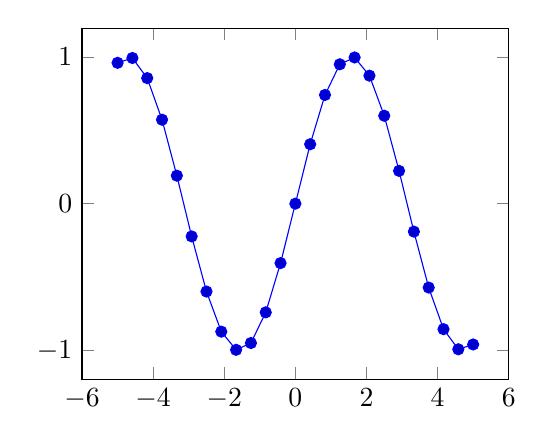
\begin{tikzpicture}
  \begin{axis}
    \addplot{sin deg(x)};
  \end{axis}
\end{tikzpicture}
\end{LTXexample}
\end{frame}

\begin{frame}[fragile,t]{Koordinaten Eingabe}
|\addplot [|\meta{Optionen}|] coordinates {|\meta{Koordinaten}|};|\vfill
\begin{LTXexample}[pos=r, explpreset={}, preset=\small, rframe={}]
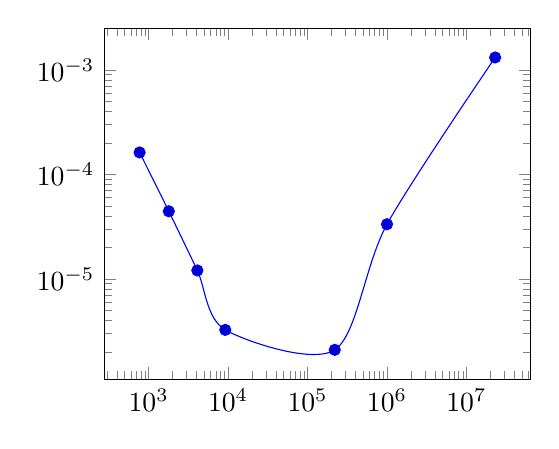
\begin{tikzpicture}
  \begin{loglogaxis}
    \addplot+[smooth]
     coordinates {
      (769, 1.6227e-04)
      (1793, 4.4425e-05)
      (4097, 1.2071e-05)
      (9217, 3.2610e-06)
      (2.2e5, 2.1E-6)
      (1e6, 0.00003341)
      (2.3e7, 0.00131415)
    };
  \end{loglogaxis}
\end{tikzpicture}
\end{LTXexample}
\end{frame}

\begin{frame}[fragile,t]{Nachbearbeitung mit \TikZ}
|\addplot [|\meta{Optionen}|] {|\meta{Eingabedaten}|} |\meta{ggf. TikZ-Befehle}|;|\vfill
\begin{LTXexample}[pos=r, explpreset={}, preset=\small, rframe={}]
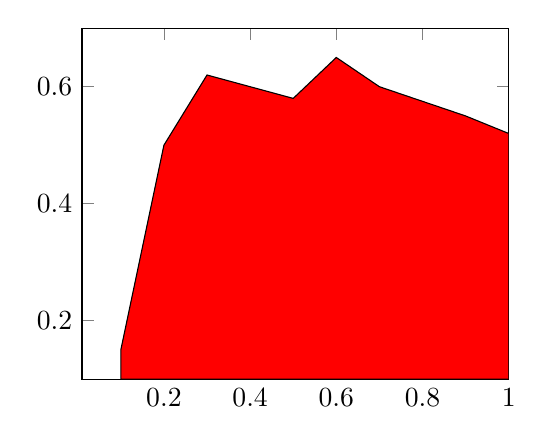
\begin{tikzpicture}
  \begin{axis}[xmax=1]
    \addplot [fill=red] coordinates
    {(0.1,0.15) (0.2,0.5)
    (0.3,0.62) (0.5,0.58)
    (0.6,0.65) (0.7,0.6)
    (0.9,0.55) (1,0.52)}
    \closedcycle;
  \end{axis}
\end{tikzpicture}
\end{LTXexample}
\end{frame}

\begin{frame}[fragile,t]{Daten-Tabellen}
|\addplot [|\meta{Optionen}|] table [|\meta{Spalten-Auswahl}|] {|\meta{Tabelle}|};|\pdfmarginpar{Tabelle kann dabei entweder eine Datei mit Tabellendaten, oder eine direkt im TeX-File eingegebe Tabelle sein.}
\vfill
\begin{LTXexample}[pos=r, explpreset={}, preset=\small, rframe={}]
\begin{tikzpicture}
  \begin{axis}
    \addplot table [
      only marks,
    ] {
      x    y    myvalue 
      0.5  0.2  0.25
      0.2  0.1  1.5
      0.7  0.6  0.75
      0.35 0.4  0.125
      0.65 0.1  2
    };
  \end{axis}
\end{tikzpicture}
\end{LTXexample}
\end{frame}


\begin{frame}[fragile,t]{Daten in externen Dateien}
|\addplot [|\meta{Optionen}|] table [|\meta{Spalten-Ausw.}|] {|\meta{Dateipfad}|};|\vfill
\begin{LTXexample}[pos=r, explpreset={}, preset=\small, rframe={}]
\begin{tikzpicture}
  \begin{axis}
    \addplot [no markers]
      table
      [x=time, y=values]
      {data.dat};
  \end{axis}
\end{tikzpicture}
\end{LTXexample}
\pause
Paket \pkg{pgfplotstable} erlaubt das Nachbearbeiten vorhandener Tabellen (z.\,B. Einfügen einer Ausgleichsgerade).
\end{frame}

\subsection{Beschriftungen}
\begin{frame}[fragile]{Beschriftungen}
\begin{tabular}{rll}
Key & Values & Funktion\\\midrule
|title| & Text & Titel über dem Diagramm\\
|x|/|ylabel| & bel. Text & Beschriftung der $x$- bzw. $y$-Achse  \\
|x|/|ymin|/|max| & Wert & schränkt Achse auf Bereich ein\\
|mark| & |*|, |x|, |+|, |o|, … & Koordinaten-Marker anpassen\\
|x|/|ytick| & Liste & Koordinatenstriche explizit angeben\\
|minor tick num| & Zahl & Anzahl der Zwischenstriche\\
|grid| & |major|, |minor| & Gitter im Hintergrund einblenden
\end{tabular}
\end{frame}

\begin{frame}[fragile,t]{Lengenden}
|\addlegendentry{|\meta{Beschreibung}|}|\vfill
\begin{LTXexample}[pos=r, explpreset={}, preset=\small, rframe={}]
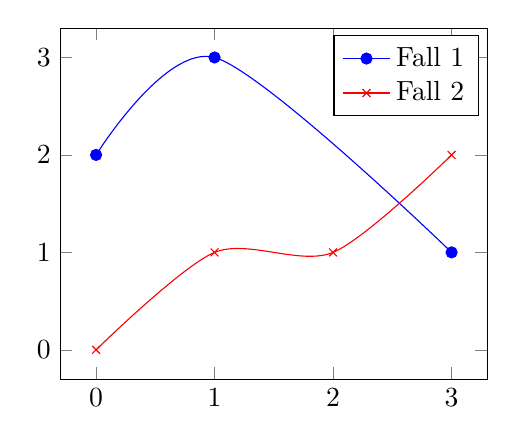
\begin{tikzpicture}
\begin{axis}
  \addplot[smooth,mark=*,blue] coordinates {
    (0,2) (1,3) (3,1)
  };
  \addlegendentry{Fall 1}
  \addplot[smooth,color=red,mark=x] coordinates {
    (0,0) (1,1) (2,1) (3,2)
  };
  \addlegendentry{Fall 2}
\end{axis}
\end{tikzpicture}
\end{LTXexample}
\end{frame}

\begin{frame}[fragile,t]{Platzierung der Achsen}
|axis y line=|\meta{Platzierung}, |axis x line=|\meta{Platzierung}\vfill
\begin{LTXexample}[pos=r, explpreset={}, preset=\small, rframe={}]
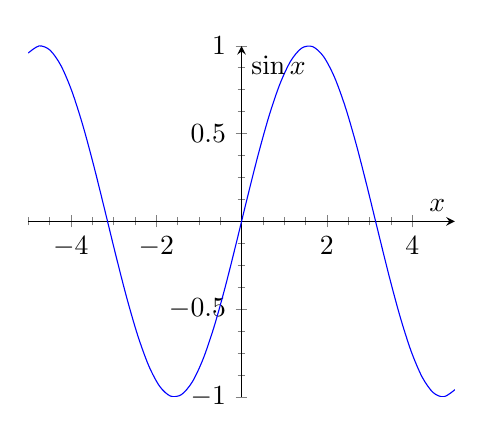
\begin{tikzpicture}
\begin{axis}[
minor tick num=3,
axis y line=center,
axis x line=middle,
xlabel=$x$,ylabel=$\sin x$
]
\addplot[smooth,blue,mark=none,
domain=-5:5,samples=40]
{sin(deg(x))};
\end{axis}
\end{tikzpicture}
\end{LTXexample}
\end{frame}

\subsection{Fehlerbalken}
\begin{frame}[fragile,t]{Fehlerbalken}
Fehler können mit den Optionen |error bars/|\meta{Key}|=|\meta{Value} gesetzt werden.\vfill
\begin{LTXexample}[pos=r, explpreset={}, preset=\small, rframe={}]
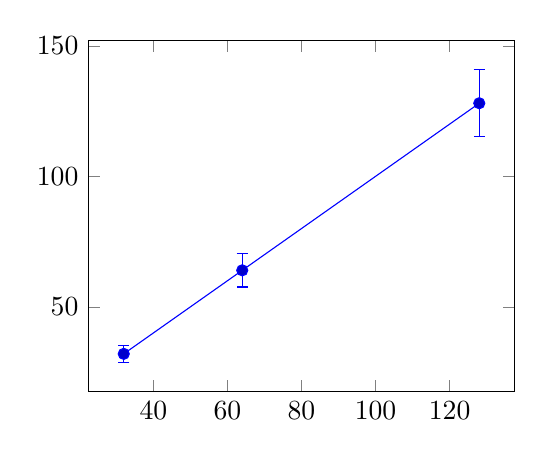
\begin{tikzpicture}
\begin{axis}
  \addplot+[
   error bars/y dir=both,
   error bars/y fixed relative=.1,
  ] table [x=x,y=y]
  {x	    y
   32     32
   64     64
   128    128
  };
\end{axis}
\end{tikzpicture}
\end{LTXexample}
\end{frame}

\begin{frame}[fragile,t]{Fehlerbalken}
Individuelle Fehler konnen mit |+-| (symmetrisch) oder |+=| und |-=| (asymmetrisch) angegeben werden:\vfill
\begin{LTXexample}[pos=r, explpreset={}, preset=\small, rframe={}]
\begin{tikzpicture}
\begin{axis}
  \addplot+[
    error bars/.cd,
    x dir=both,
    x explicit,
    y dir=both, 
    y explicit,
  ] coordinates {
    (1,1) += (0.4,0.2) 
          -= (0.1,0.1)
    (3,2) -= (1,0)
    (4,5) +- (0.3,0.2)
  };
\end{axis}
\end{tikzpicture}
\end{LTXexample}
\end{frame}

\begin{frame}[fragile,t]{Fehlerbalken}
Fehler können auch aus einer Tabelle stammen:\vfill
\begin{LTXexample}[pos=r, explpreset={}, preset=\small, rframe={}]
\begin{tikzpicture}
  \begin{axis}
    \addplot [only marks, mark=x, 
    error bars/.cd,
    y dir=both, y explicit,]
      table
      [x=time, y=values, y error=error]
      {data.dat};
  \end{axis}
\end{tikzpicture}
\end{LTXexample}
\end{frame}



\subsection{Histogramme}
\begin{frame}[fragile,t]{Histogramme}
Histogramme mit Option |hist={|\meta{Histogram-Optionen}|}|\vfill
\begin{LTXexample}[pos=r, explpreset={}, preset=\small, rframe={}]
\begin{tikzpicture}
  \begin{axis}
    \addplot+[
      fill=blue!40!white,
      mark={},
      hist={
        data=y, 
        bins=10
      }
    ] table {data.dat};
  \end{axis}
\end{tikzpicture}
\end{LTXexample}
Interessante Optionen:\\|cummulative| für kummuliertes Histogram\\|density| normiert auf 1
\end{frame}

\subsection{Balkendiagramme}
\begin{frame}[fragile,t]{Balkendiagramme}
Option |xbar| erzeug Balkendiagramm, |ybar| erzeugt Säulendiagramm\vfill
\begin{LTXexample}[pos=r, explpreset={}, preset=\small, rframe={}]
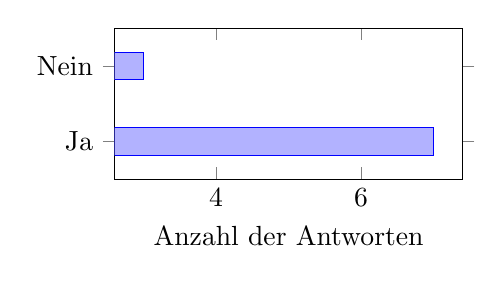
\begin{tikzpicture}
\begin{axis}[
 xbar,
 width=6cm, height=3.5cm,
 enlarge y limits=0.5,
 xlabel={Anzahl der Antworten},
 symbolic y coords={Ja,Nein},
 ytick=data,
]
 \addplot coordinates
  {(3,Nein) (7,Ja)};
\end{axis}
\end{tikzpicture}
\end{LTXexample}
\end{frame}

\subsection{Balkendiagramme}
\begin{frame}[fragile,t]{Balkendiagramme}
Option |xbar| erzeug Balkendiagramm, |ybar| erzeugt Säulendiagramm\vfill
\begin{LTXexample}[pos=r, explpreset={}, preset=\small, rframe={}]
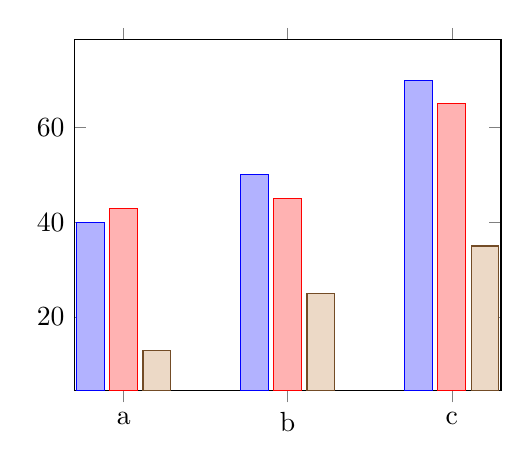
\begin{tikzpicture}
\begin{axis}[
 ybar,enlargelimits=0.15,
 symbolic x coords={a,b,c},xtick={a,b,c},
]
 \addplot coordinates 
 {(a,40) (b,50) (c,70)};
 \addplot coordinates 
 {(a,43) (b,45) (c,65)};
 \addplot coordinates 
 {(a,13) (b,25) (c,35)};
\end{axis}
\end{tikzpicture}
\end{LTXexample}
\end{frame}



\subsection{Boxplots}
\begin{frame}[fragile,t]{Boxplots}
|\usepgfplotslibrary{statistics}| erlaubt Satz von Boxplots:\vfill
\usepgfplotslibrary{statistics}
\begin{LTXexample}[pos=r, explpreset={}, preset=\small, rframe={}]
\begin{tikzpicture}
  \begin{axis}
    \addplot+[
    boxplot prepared={
      median=4000,
      upper quartile=5500,
      lower quartile=3000,
      upper whisker=1200,
      lower whisker=15000,
    } ] coordinates {};
  \end{axis}
\end{tikzpicture}
\end{LTXexample}
\end{frame}


\subsection{Polarkoordinaten}
\begin{frame}[fragile,t]{Polarkoordinaten}
Mit |\usepgfplotslibrary{polar}| versteht \pkg{pgfplots} Polarkoordinaten.\\
|polaraxis| geht von Polarkoordinaten aus:\vfill
\begingroup
\pgfplotsset{scale=0.9}
\usepgfplotslibrary{polar}
\begin{LTXexample}[pos=r, explpreset={}, preset=\small, rframe={}]
\begin{tikzpicture}
  \begin{polaraxis}
    \addplot coordinates {(90,1) (180,1)};
  \end{polaraxis}
\end{tikzpicture}
\end{LTXexample}
\endgroup
\end{frame}


\subsection{gnuplot}
\begin{frame}[fragile,t]{gnuplot in pgfplots}
|\addplot gnuplot [|\meta{Optionen}|] {|\meta{gnuplot Befehle}|};|\vfill

\begin{LTXexample}[pos=r, explpreset={}, preset=\small, rframe={}]
\begin{tikzpicture}
  \begin{semilogyaxis}
    \addplot gnuplot
      [domain=0:10]
      {exp(x)};
  \end{semilogyaxis}
\end{tikzpicture}
\end{LTXexample}
\end{frame}

\begin{frame}[fragile,t]{gnuplot in |pgfplots|}
|\addplot gnuplot [|\meta{Optionen}|] {|\meta{gnuplot Befehle}|};|\vfill
\begin{itemize}
\item \pkg{pgfplots} ruft gnuplot auf und speichert das Ergebnis in Hilfsdateien. 
\item gnuplot wird nur aufgerufen, wenn sich etwas geändert hat.
\item gnuplot ist etwas schneller als interne Plots.
\item gnuplot stellt mehr mathematische Funktionen zur Verfügung.
\item gnuplot nutzt Radiant für Winkel, \pkg{pgfplots} nutzt Grad\\(außer mit Einstellung |trig format=rad|).
\item gnuplot und interne Plots haben etwa die selbe Genauigkeit.
\end{itemize}
\end{frame}



\subsection{3D-Plots}
\begin{frame}[fragile,t]{3D-Plots}% \verb|\textbackslash addplot3|}
|\addplot3 [|\meta{Optionen}|] {|\meta{Eingabedaten}|};| \vfill
\begin{LTXexample}[pos=r, explpreset={}, preset=\small, rframe={}]
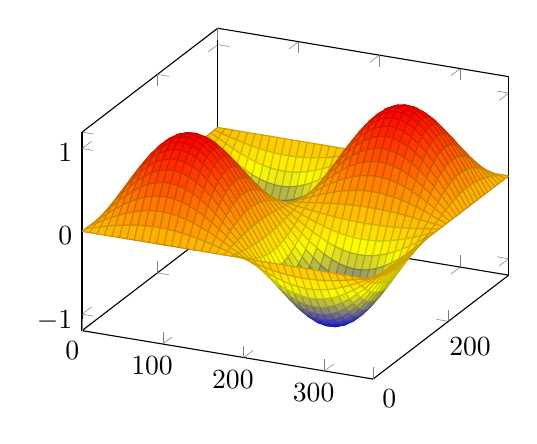
\begin{tikzpicture}
  \begin{axis}
    \addplot3[
      surf,
      domain=0:360,
      samples=40,
    ]
    {sin(x)*sin(y)};
  \end{axis}
\end{tikzpicture}
\end{LTXexample}
\end{frame}



%% Plots
%%   achsenbeschriftungen
%%   achse verschieben
%%   grids



\begin{frame}{Was |pgfplots| noch so alles kann …}
\begin{itemize}
\item extern erzeugte Plots (Bilder) in pgfplot-Koordinatensystem einfügen (auch 3D)
\item in Matlab erzeugte Plot importieren
\item beliebige Befehle in einer Shell ausführen und das Ergebnis plotten
\item Datum oder Uhrzeit als Koordinaten
\item automatische Umrechnung von Koordinaten (z.\,B. polar in kartesisch)
\item klickbare Plots (die ein Popup öffnen)
\item Plots in einzelne externe Dateien ausgeben
\item Flächen zwischen Kurven schraffieren
\item Vektorfelder plotten
\item Alle Diagramme als einzelne PDF generieren, um diese nicht immer wieder neu generieren zu müssen
\item …
\item alles was \TikZ\ kann
\end{itemize}
\end{frame}

\nocite{pgfplots}
\begin{frame}[allowframebreaks]{Weiterführende Literatur}
\printbibliography
\end{frame}

\end{document}
